% -*- TeX:de -*-
\NeedsTeXFormat{LaTeX2e}
\documentclass[12pt,a4paper]{article}
\usepackage[german]{babel} % german text
\usepackage[DIV12]{typearea} % size of printable area
\usepackage[T1]{fontenc} % font encoding
%\usepackage[latin1]{inputenc} % most likely on Windows
\usepackage[utf8]{inputenc} % probably on Linux
\usepackage{multicol}

% PLOTTING
\usepackage{pgfplots} 
\usepackage{pgfplotstable}
\usepackage{url}
\usepackage{graphicx} % to include images
\usepackage{tikz}
\usepackage{subfigure} % for creating subfigures
\usepackage{amsmath} % a bunch of symbols
\usepackage{amssymb} % even more symbols
\usepackage{booktabs} % pretty tables
\usepackage{makecell} % multi row table heading

% a floating environment for circuits
\usepackage{float}
\usepackage{caption}

%\newfloat{circuit}{tbph}{circuits}
%\floatname{circuit}{Schaltplan}

% a floating environment for diagrams
%\newfloat{diagram}{tbph}{diagrams}
%\floatname{diagram}{Diagramm}
\pgfplotsset{compat=1.8}
\selectlanguage{german} % use german

\begin{document}

%%%%%%% DECKBLATT %%%%%%%
\thispagestyle{empty}
			\begin{center}
			\Large{Fakultät für Physik}\\
			\end{center}
\begin{verbatim}


\end{verbatim}
							%Eintrag des Wintersemesters
			\begin{center}
			\textbf{\LARGE SS 14}
			\end{center}
\begin{verbatim}


\end{verbatim}
			\begin{center}
			\textbf{\LARGE{Physikalisches Praktikum\\ für das Bachelorstudium}}
			\end{center}
\begin{verbatim}




\end{verbatim}

			\begin{center}
			\textbf{\LARGE{PROTOKOLL}}
			\end{center}
			
\begin{verbatim}

\end{verbatim}

			\begin{flushleft}
			\textbf{\Large{Experiment (Nr., Titel): PS3 - Radioaktivität}\\
							%Experiment Nr. und Titel statt den Punkten eintragen
			\LARGE{PS3}}	
			\end{flushleft}

\begin{verbatim}

\end{verbatim}	
							%Eintragen des Abgabedatums, oder des Erstelldatums des Protokolls
			\begin{flushleft}
			\textbf{\Large{Datum:}} \Large{26.06.2014}
			\end{flushleft}
			
\begin{verbatim}
\end{verbatim}
							%Namen der Protokollschreiber
		\begin{flushleft}
			\textbf{\Large{Namen:}} \Large{Patrick Braun, Johannes Kurz}
			\end{flushleft}

\begin{verbatim}


\end{verbatim}
							%Kurstag und Gruppennummer, zb. Fr/5
			\begin{flushleft}
			\textbf{\Large{Kurstag/Gruppe:}} \Large{DO/4}
			\end{flushleft}

\begin{verbatim}

\end{verbatim}
							%Name des Betreuers, das Praktikum betreute.
			\begin{flushleft}
			\LARGE{\textbf{Betreuer:}}	\Large{Jonas Rodewald}	
			\end{flushleft}

%%%%%%% DECKBLATT ENDE %%%%%%%
\pagebreak
\setlength{\columnsep}{20pt}
\begin{multicols}{2}

%%%%%%%%%%%%%%%%%%%%%%%%%%%%%%%%%%%%%%%%%%%%%%%%

%\begin{figure}[H]
%	\centering
%	\includegraphics[scale=0.35]{./figure/beugung.png}
%	\caption{Beugungsmuster Einzelspalt (echtes Foto; schwarz durch weiß ersetzt)}
%	\label{fig:beugungsmuster}
%\end{figure}


%\begin{figure}[H]
%	\centering
%	\pgfplotstabletypeset[
%			columns={abstand, n},
%			col sep=&,
%			columns/abstand/.style={precision=2, zerofill, column name=\makecell{$Abstand$\\$(\pm 0.05)[mm]$} }, 
%			columns/n/.style={column name=\makecell{$n$\\$(Ordnung)$}, precision=0},
%			every head row/.style={before row=\hline,after row=\hline\hline},
%			every last row/.style={after row=\hline},
%			every first column/.style={column type/.add={|}{} },
%			every last column/.style={column type/.add={}{|} }
%			]{
%			abstand & n
%			12.9 & 1
%			24.45 & 2
%			37.40 & 3
%			49.35& 4
%			62.45 & 5
%			74.45 & 6
%			87.45 & 7
%			100.25 & 8
%			
%			}
%	\caption{Messwerte Einzelspalt}
%	\label{tab:werte_einzelspalt}
%\end{figure}


%%%%%%%%%%%%%%%%%%%%%%%%%%%%%%%%%%%%%%%%%%%%%%%%
%%%%%%%%%%%%%%%%%%%%%%%%%%%%%%%%%%%%%%%%%%%%%%%%


%\section{Schwingungen 2}
\noindent In PS3 werden die verschiedenen Arten von Radioaktivität untersucht. In den folgenden Versuchen werden einige Fragestellungen zu $\alpha-, \beta- und \gamma-Strahlung$ durch ausgewählte Experimente beantwortet.

%%%%%%%%%%%%%%%%%%%%%%%%%%%%%%%%%%%%%%%%%%%%%%%%%%%%%%%%%%%%%%%%%%%%%%%
\section{Grundlagen}
Es werden drei Arten von Strahlung unteschieden ([1] p.2):
\begin{itemize}
	\item $\alpha-Strahlung$: 2-fach positiv geladene Helliumkerne
	\item $\beta-Strahlung$: Elektronen oder Positronen; hauptsächlich künstliche Radioaktive Elemente; weitere Zerfälle
	\item $\gamma-Strahlung$ hochenergetische Photonen (entstehen bei $\alpha-$ und $\beta-Zerfällen$)
\end{itemize}
Der Zerfall ist für gleiche Elemente gleich wahrscheinlich. 
Daher kann ein einfachs Zerfallsgesetzt abhängig von der Gesamtanzahl der betrachteten Atome formuliert werden.
\subsection{Radioaktiver Zerfall von Kupfer}
$$\frac{dN(t)}{dt} = -\lambda N(t)$$
\subsection{Beta- und Gammaspektroskopie}

\subsection{Abstandsgesetz für punktförmige Strahler}

\subsection{Reichweite von Alpha-Strahlen in Luft}


%%%%%%%%%%%%%%%%%%%%%%%%%%%%%%%%%%%%%%%%%%%%%%%%%%%%%%%%%%%%%%%%%%%%%%%
\pagebreak
\section{Versuchsaufbau:}



\subsection{Radioaktiver Zerfall von Kupfer}

\subsection{Beta- und Gammaspektroskopie}

\subsection{Abstandsgesetz für punktförmige Strahler}

\subsection{Reichweite von Alpha-Strahlen in Luft}


%%%%%%%%%%%%%%%%%%%%%%%%%%%%%%%%%%%%%%%%%%%%%%%%%%%%%%%%%%%%%%%%%%%%%%%
\pagebreak
\section{Resultate}
\subsection{Radioaktiver Zerfall von Kupfer}
\begin{figure}[H]
	\centering
	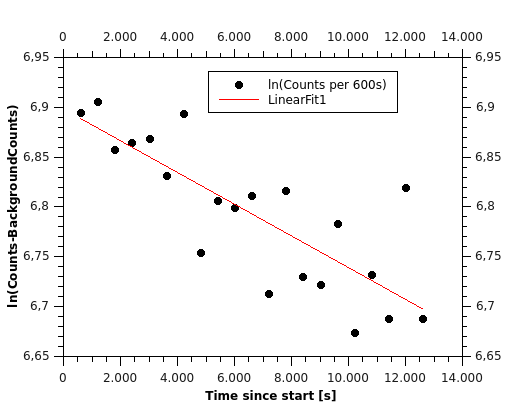
\includegraphics[scale=1.5]{./figures/kupfer_zerfall_ergebnis.png}
	\caption{Logarithmus der Aktivität gegen Zeit, Steigung entspricht $\lambda$}
	\label{fig:kupferzerfall_erg}
\end{figure}
% $\lambda$ = (-1.591120669338278 \pm 0.2686603661676406) E-05
 $\lambda = (-1.6 \pm 0.3) E-5$\\
 $\tau = (17.46 \pm 2.43)h$\\
 %(ln(2)/0.00001591120669338278)/60/60
 $$T_{1/2} = (12.1 \pm 2.1)h$$
 $$T_{1/2} ({64}^Cu) = 12.701(2) h$$
 Quelle: [3]
\subsection{Beta- und Gammaspektroskopie}

\subsection{Abstandsgesetz für punktförmige Strahler}

Peak 1: 1117keV bis 1256keV\\
Peak 2: 1260keV bis 1409keV\\
Abstände: 5.5cm, 6cm, 7cm, 9cm, 13cm\\
\begin{figure}[H]
	\centering
	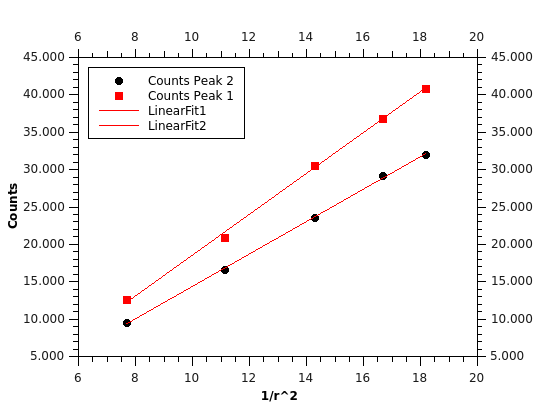
\includegraphics[scale=1.5]{./figures/Endergebniss_Abstand_mitFits.png}
	\caption{Verhältnis von Abstand ($r^2$) zu Ereignisanzahl (ln von Summe über Bereich)}
	\label{fig:abstandsgesetz_erg}
\end{figure}
% TODO lambda? für echte Countes vom intercept e^intercept ;)

% [30.06.14 21:45	Diagramm: ''Grafik1'']
% Lineare Regression von Datensatz: FitIntegralergebnisse_ln(Counts1), unter Verwendung der Funktion: A*x+B
% Gewichtungsmethode: Keine Gewichtung (alle w_i = 1)
% Von x = 5,500000000000000e-02 bis x = 1,300000000000000e-01
% B (y-intercept) = 1,144194727689966e+01 +/- 8,079573075641884e-02
% A (slope) = -1,570157544300322e+01 +/- 9,453188177227960e-01
% --------------------------------------------------------------------------------------
% Chi^2/doF = 3,324294921763869e-03
% R^2 = 0,989242921157287
% Angepasstes R^2 = 0,978485842314573
% RMSE (Standardabweichung) = 0,0576566988455274
% RSS (Summe der quadrierten Restwerte) = 0,00997288476529153
% ---------------------------------------------------------------------------------------
% [30.06.14 21:45	Diagramm: ''Grafik1'']
% Lineare Regression von Datensatz: FitIntegralergebnisse_ln(Counts2), unter Verwendung der Funktion: A*x+B
% Gewichtungsmethode: Keine Gewichtung (alle w_i = 1)
% Von x = 5,500000000000000e-02 bis x = 1,300000000000000e-01
% B (y-intercept) = 1,122650811491831e+01 +/- 6,738920842337341e-02
% A (slope) = -1,613655635448036e+01 +/- 7,884610515636363e-01
% --------------------------------------------------------------------------------------
% Chi^2/doF = 2,312615486978147e-03
% R^2 = 0,992888511500226
% Angepasstes R^2 = 0,985777023000453
% RMSE (Standardabweichung) = 0,048089660915608
% RSS (Summe der quadrierten Restwerte) = 0,00693784646093448
% ---------------------------------------------------------------------------------------
\subsection{Reichweite von Alpha-Strahlen in Luft}



%%%%%%%%%%%%%%%%%%%%%%%%%%%%%%%%%%%%%%%%%%%%%%%%%%%%%%%%%%%%%%%%%%%%%%%
\pagebreak
\section{Diskussion}

\subsection{Radioaktiver Zerfall von Kupfer}

\subsection{Beta- und Gammaspektroskopie}

\subsection{Abstandsgesetz für punktförmige Strahler}

\subsection{Reichweite von Alpha-Strahlen in Luft}



%%%%%%%%%%%%%%%%%%%%%%%%%%%%%%%%%%%%%%%%%%%%%%%%%%%%%%%%%%%%%%%%%%%%%%%
\section{Quellen}
$[1]$ Anleitung, \url{http://www.univie.ac.at/anfpra/neu1/ps/ps3/PS3.pdf}\\
$[2]$ Rohdaten, \url{htts://github.com/blackandcold/Protocols-SS2014-P2/tree/master/PS_3/data}\\
$[3]$ Kupfer, \url{http://www.internetchemie.info/chemiewiki/index.php?title=Kupfer-Isotope}
\end{multicols}
\end{document}